Acest capitol va descrie detaliat algoritmul de modelare acustic\u{a} \^{i}n spa\c{t}ii interioare folosind metoda Ray-Tracing \c{s}i va con\c{t}ine pa\c{s}ii elementari pentru implementarea acestuia. \c{T}in\^{a}nd cont de toate acestea, aplica\c{t}ia poate fi \^{i}mp\u{a}r\c{t}it\u{a} \^{i}n patru etape:
\begin{enumerate}
	\utb Calcul geometric
	\begin{itemize}
		\item Sfera lui Fibonacci - este un algoritm ce presupune distribuirea punctelor în mod uniform pe suprafața unei sfere
		\item Propagarea razelor - presupune distribuirea unui număr finit de raze în încăpere pornind de la niște puncte de start și ținând cont de numărul maxim de reflexii pe care îl poate avea o rază și de distanța maximă a acesteia
		\item Selec\c{t}ia razelor - dintr-un număr cunoscut de raze se vor selecta doar acelea care îndeplinesc anumite condiții
	\end{itemize}
	\utb Calcul fizic
	\begin{itemize}
		\item Calculul intensit\u{a}\c{t}ilor - pentru fiecare punct de coliziune al unei raze trebuie calculată intensitatea ținând cont de suprafețele de impact
		\item Calculul presiunilor - fiecare intensitate calculată la pasul anterior trebuie transformată în presiune ținând cont de temperatura din mediu, viteza sunetului prin aer și de densitatea aerului
		\item Func\c{t}ia de r\u{a}spuns la frecven\c{t}\u{a} \c{s}i func\c{t}ia de r\u{a}spuns la impuls - este necesar să cunoaștem valorile acestor funcții pentru a putea obține rezultatele finale
		\item Calculul distan\c{t}elor - pentru fiecare rază trebuie să cunoaștem lungimea acesteia
		\item Calculul timpilor - pentru fiecare rază trebuie să cunoaștem momentul la care aceasta a lovit un anumit obiect, în cazul acestui studiu obiectul de interes este microfonul
	\end{itemize}
	\utb Post-procesare 
	\begin{itemize}
		\item Convolu\c{t}ia sunetului - presupune preluarea funcției de răspuns la impuls și a sunetului care a fost difuzat în încăpere si combinarea acestora pentru a obține soluția
	\end{itemize}
	\utb GUI (Graphical User Interface)
\end{enumerate}
 

Astfel, pentru a realiza acest model trebuie s\u{a} \^{i}ncepem prin a distribui uniform razele plec\^{a}nd de la surs\u{a}, dup\u{a} care trebuie s\u{a} select\u{a}m razele care intersecteaz\u{a} microfoanele din \^{i}nc\u{a}pere. Pentru a ob\c{t}ine performan\c{t}\u{a} este necesar s\u{a} excludem acele raze care nu ajung pe nici unul dintre microfoane sau acele raze care intersecteaz\u{a} microfoanele, dar sunt foarte asem\u{a}n\u{a}toare \c{s}i s\u{a} pastr\u{a}m doar una dintre aceste raze asemănătoare pentru a reduce din costul computațional.

 
Pentru pasul urm\u{a}tor calcul\u{a}m intensit\u{a}\c{t}ile pentru fiecare raz\u{a} pe care mai apoi le transform\u{a}m \^{i}n presiuni. Urm\u{a}toarea etap\u{a} presupune calculul frecven\c{t}elor \c{s}i calcularea fazelor. Dup\u{a} ce ace\c{s}ti pa\c{s}i au fost realizați, mai este nevoie doar s\u{a} calcul\u{a}m distan\c{t}ele \c{s}i timpii pentru ca mai departe s\u{a} ob\c{t}inem func\c{t}ia de r\u{a}spuns la impuls \c{s}i func\c{t}ia de r\u{a}spuns în frecven\c{t}\u{a}.

  
Acum c\u{a} am considerat toate aceste etape mai rămâne doar s\u{a} putem interpreta rezultatul algoritmului nostru. Astfel, cu ajutorul convolu\c{t}iei ajungem s\u{a} ascult\u{a}m solu\c{t}ia algoritmului, iar modelul nostru acustic este complet.

\section{Ghid de utilizare al aplica\c{t}iei}

	Acustica face parte din domeniul fizicii \c{s}i se ocup\u{a} cu studiul undelor mecanice \^{i}n gaze, lichide, solide \c{s}i este prezent \^{i}n toate aspectele societ\u{a}\c{t}ii actuale, \^{i}ns\u{a} predominant \^{i}n domeniul industriei pentru controlul zgomotului. Aceast\u{a} ramur\u{a} implic\u{a} \c{s}i studiul sunetelor, vibra\c{t}iilor, ultrasunetelor \c{s}i infrasunetelor. Un model acustic va implica, \^{i}n cel mai generic mod, simularea c\u{a}ilor pe care sunetul le parcurge de la surs\u{a} la destina\c{t}ie. Cel mai adesea, aceste modele presupun rezolvarea integralei Helmoltz-Kirchoff \cite{helmoltz} folosind diverse abord\u{a}ri de calcul, precum: solu\c{t}ii numerice ale ecua\c{t}iei de und\u{a}, aproxim\u{a}ri de \^{i}nalt\u{a} frecven\c{t}\u{a} ale ecua\c{t}iei de und\u{a}, dar \c{s}i modele statistice. Modelul pe care \^{i}l propune acest studiu face parte din cea de-a doua categorie. Modelul acustic va con\c{t}ine etapa de calcul geometric, etapa de calcul fizic, convolu\c{t}ia sunetului \c{s}i realizarea unei interfe\c{t}e ce permite validarea acestor rezultate.
	 
	
	\c{T}in\^{a}nd cont de toate aceste elemente este foarte important s\u{a} re\c{t}inem c\u{a} aceste etape se afl\u{a} \^{i}ntr-o leg\u{a}tur\u{a} str\^{a}ns\u{a} \c{s}i se bazeaz\u{a} unele pe celelalte. Astfel, ne putem da seama c\u{a} calculul geometric este o etap\u{a} deosebit de important\u{a}, \^{i}ntruc\^{a}t modul \^{i}n care distribuim razele \^{i}n \^{i}nc\u{a}pere \c{s}i selec\c{t}ia acestora dicteaz\u{a} performan\c{t}a modelului \c{s}i optimalitatea acestuia. Algoritmii de post-procesare sunt folosi\c{t}i, de obicei, pentru a suprima zgomotul sau orice artefact creat \^{i}n cadrul primelor dou\u{a} etape, adic\u{a} calculul geometric \c{s}i cel fizic, concentr\^{a}ndu-se pe eliminarea distorsiunii \c{s}i a ecoului.
	
	Aplicația dezvoltată în această lucrare cuprinde toate etapele enunțate mai sus și urmează a fi detaliate în paginile ce urmează. Pentru început va fi prezentat modul în care arată aplicația și funcționalitățile acesteia, urmând să fie prezentat și modul în care a fost creat modelul acustic.
	
	Interfa\c{t}a aplica\c{t}iei a fost realizat\u{a} cu ajutorul platformei Unity. \^{I}nc\u{a}perile dreptunghiulare au fost construite folosind formele 3D puse la dispozi\c{t}ie de c\u{a}tre aceast\u{a} platform\u{a}, iar \^{i}nc\u{a}perea sferic\u{a} a fost creat\u{a} \^{i}n Blender. Pentru cea din urm\u{a} camer\u{a} a fost folosit un obiect de tip sfer\u{a} pentru care au fost inversate normalele. Fiecare spa\c{t}iu folose\c{s}te culori \c{s}i materiale potrivite utiliz\^{a}nd Unity Material, o clas\u{a} care permite utilizatorului s\u{a} animeze un obiect prin intermediul propriet\u{a}\c{t}ilor de care dispune aceast\u{a} clas\u{a}.
	
	Pentru acest studiu au fost g\^{a}ndite trei \^{i}nc\u{a}peri: dou\u{a} dreptunghiulare \c{s}i una sferic\u{a}. Prima \^{i}nc\u{a}pere dreptunghiular\u{a} are dimenisunea de 4x5m, iar cea de-a doua are 30x30m. \^{i}nc\u{a}perea sferic\u{a} are raza 5m. Acestea pot fi vizualizate \^{i}n Figura \ref{rooms}. Pentru \^{i}nc\u{a}perile dreptunghiulare sursa a fost pozi\c{t}ionat\u{a} \^{i}n centru, iar pentru \^{i}nc\u{a}perea sferic\u{a} sursa a fost pozitionat\u{a} astfel \^{i}nc\^{a}t s\u{a} apar\c{t}in\u{a} unui cerc pe care vor fi plasate microfoanele. Formele încăperilor au fost alese pentru a reprezenta o parte din formele de bază pe care o încăpere le poate avea.
	
	\begin{figure}[!htb]%
		\begin{subfigure}[b]{.3\textwidth}
			\centering
			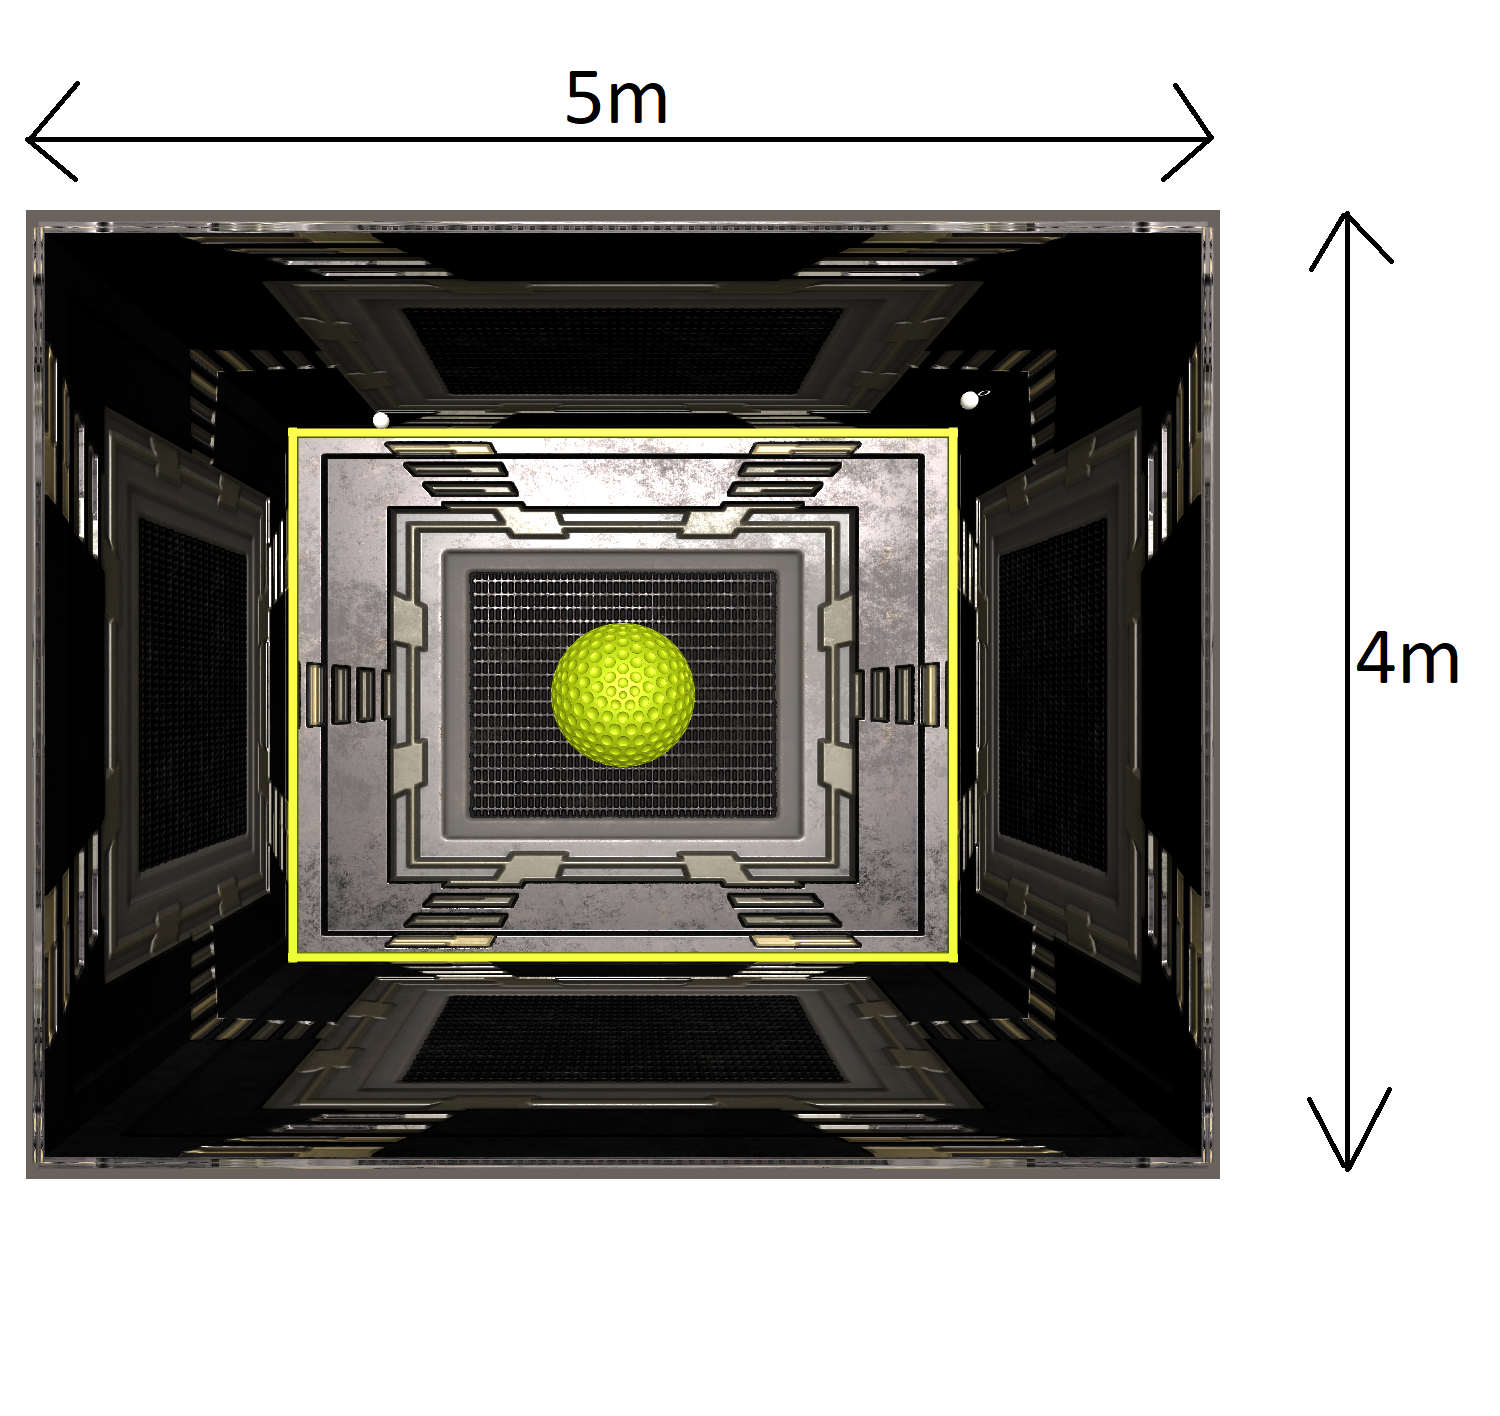
\includegraphics[width=1\linewidth]{imagini/smallRoom.png} 
			\caption{\^{I}nc\u{a}perea dreptunghiular\u{a} mic\u{a}}
			%\label{fig:sub-fig}
		\end{subfigure}
		\hfill
		\begin{subfigure}[b]{.3\textwidth}
			\centering
			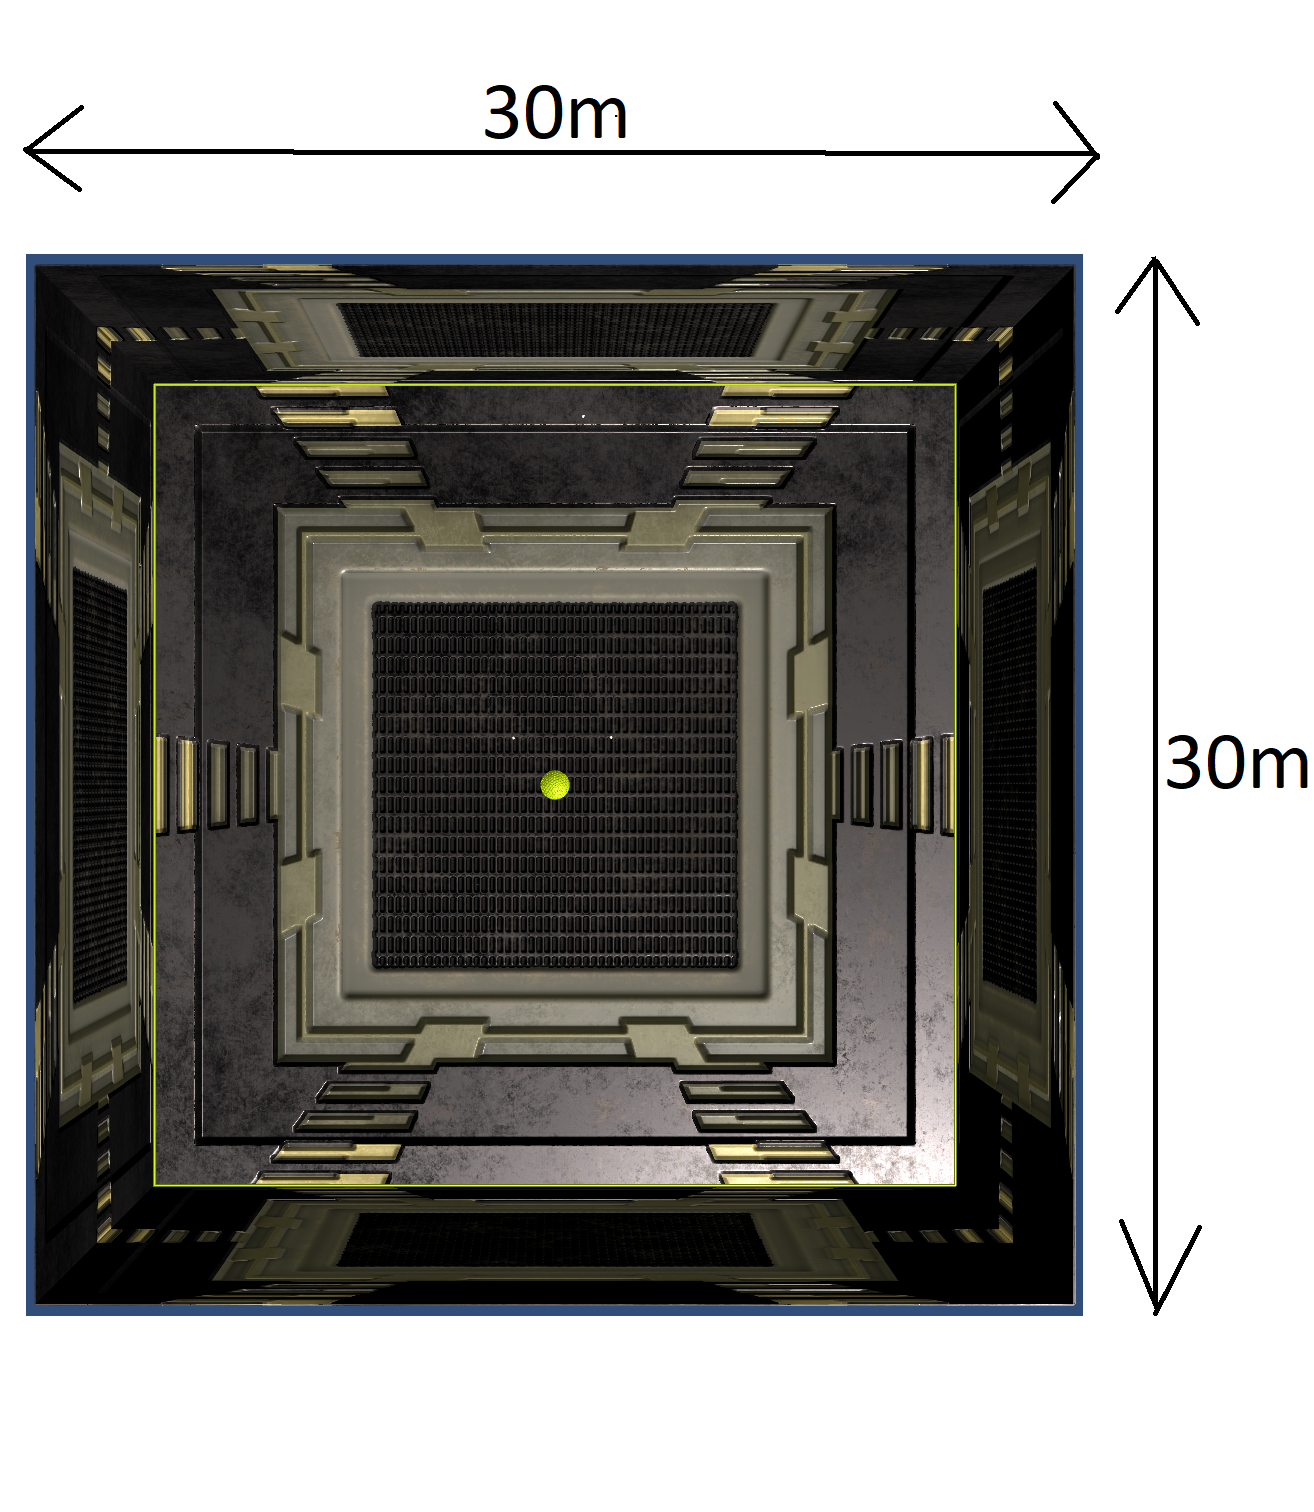
\includegraphics[width=1\linewidth]{imagini/bigRoom.png}
			\caption{\^{I}nc\u{a}perea dreptunghiular\u{a} mare}
			%\label{fig:sub-second}
		\end{subfigure}
		\hfill
		\begin{subfigure}[b]{.3\textwidth}
			\centering
			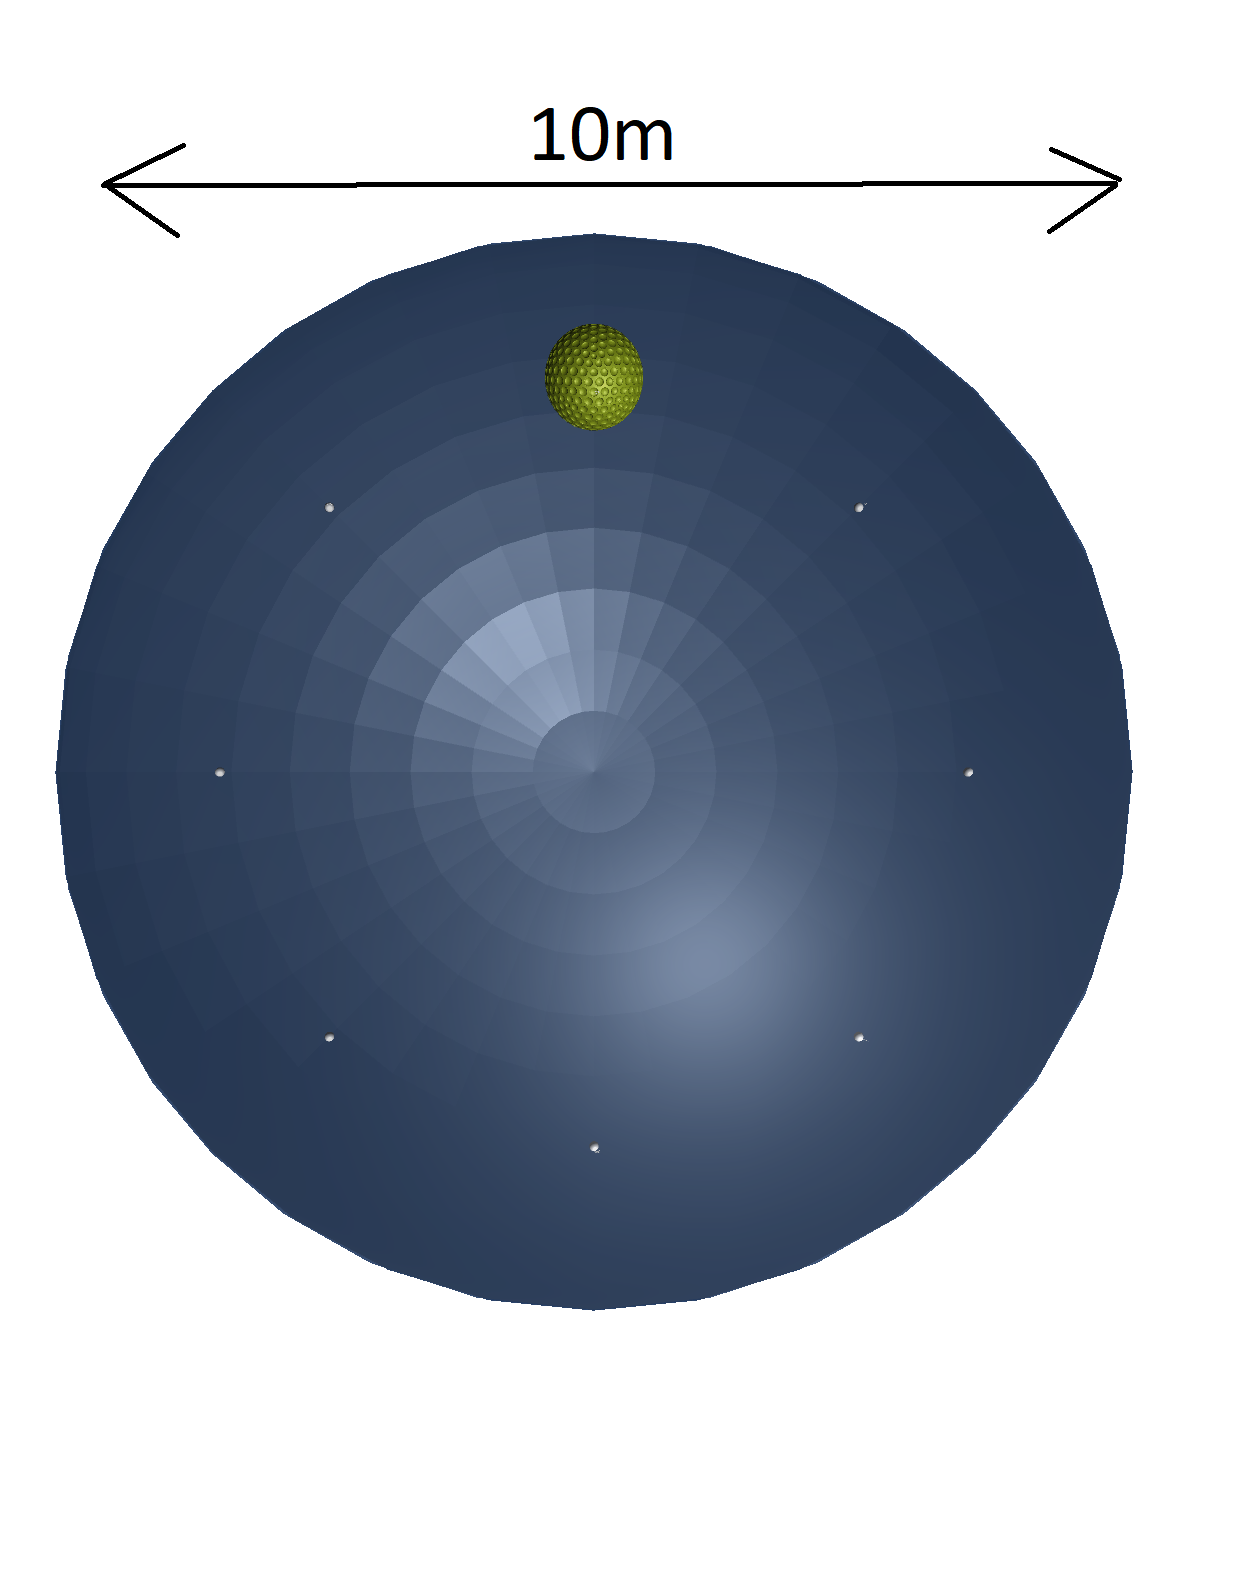
\includegraphics[width=1\linewidth]{imagini/sphericRoom.png}
			\caption{\^{I}nc\u{a}perea sferic\u{a}}
			%\label{fig:sub-third}
		\end{subfigure}
		
		\caption{Tipuri de încăperi studiate}
		\label{rooms}
	\end{figure}
	
	 
	Meniurile aplica\c{t}iei au fost realizate tot cu ajutorul platformei Unity folosind elemente de UI precum: Canvas, Panel, Button, Dropdown, Label, Input, Text, dar \c{s}i altele. Canvas-ul este un element ce con\c{t}ine o arie \^{i}n interiorul c\u{a}reia ar trebui s\u{a} se afle toate celelalte elemente de UI, iar un Panel este utilizat pentru a sus\c{t}ine mai multe elemente precum Button, Label, Input, Dropdown, Text etc. De asemenea, pentru butoane au fost alese imagini intuitive care s\u{a} u\c{s}ureze folosirea acestora, dar \c{s}i un font adecvat pentru text astfel \^{i}nc\^{a}t s\u{a} fie lizibil pentru utilizator.
	
	Aplicația conține un meniu principal care permite selecția camerei pe care dorim să o alegem, dar și un buton de exit. După ce intrăm în una dintre încăperi vom avea posibilitatea să ne plimbăm prin cameră sau să alegem una dintre cele 3 opțiuni: deschiderea meniului ce setează datele de intrare pentru modelul acustic, rularea acestuia și observarea rezultatelor; deschiderea meniului pentru vizualizarea tuturor razelor sau vizualizarea unei singure raze; butonul de back care permite alegerea unei alte camere.
	
	\begin{figure}[!htb]
		\centering
		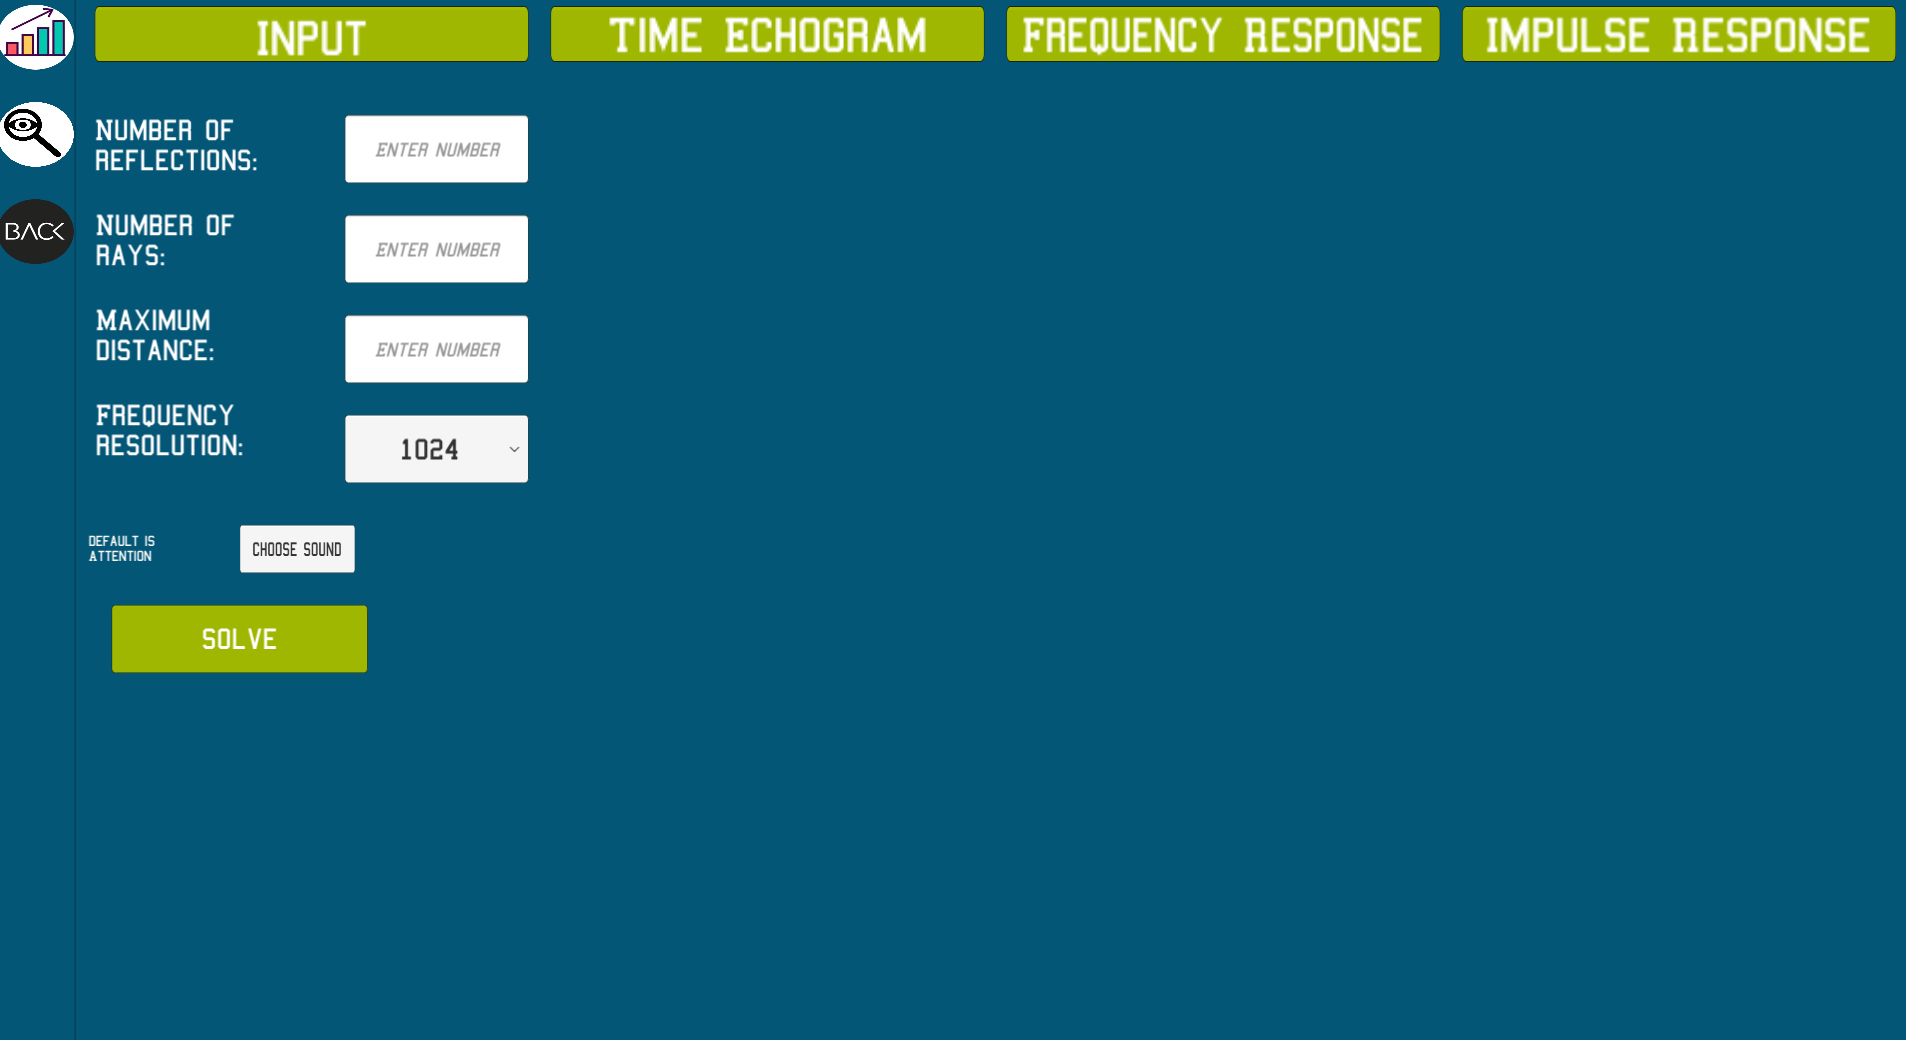
\includegraphics[width=1\linewidth]{imagini/input.png}
		\caption{Meniul pentru setarea configura\c{t}iei}
		\label{inputFig}
	\end{figure}

	\^{I}n Figura \ref{inputFig} putem observa meniul care ne ajut\u{a} s\u{a} set\u{a}m valorile pentru care dorim s\u{a} analizăm ce se \^{i}nt\^{a}mpl\u{a} \^{i}ntr-o \^{i}nc\u{a}pere cu sunetul. Cu ajutoul acestei ferestre avem posibilitatea de a parametriza algoritmul \c{s}i putem stabili care este num\u{a}rul maxim de reflexii permis pentru o raz\u{a}, num\u{a}rul de raze ce se vor \^{i}mpr\u{a}\c{s}tia \^{i}n camer\u{a}, distan\c{t}a maxim\u{a} permis\u{a} pentru o raz\u{a}, pasul de frecvență \c{s}i sunetul ce va fi difuzat \^{i}n \^{i}nc\u{a}pere. De asemenea, flexibiltatea aplicației este sporită prin includerea celor 3 ferestre: \textit{TIME ECHOGRAM, FREQUENCY RESPONSE} \c{s}i \textit{IMPULSE RESPONSE}, oferind o gamă variată de a vizualiza \c{s}i interpreta rezultatele.
	 
	
	\begin{figure}[!htb]
		\centering
		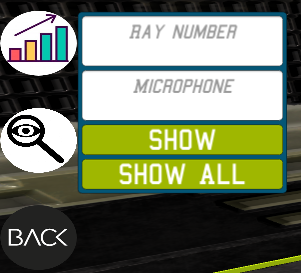
\includegraphics[width=6cm]{imagini/rayMenu.png}
		\caption{Meniul pentru vizualizarea razelor}
		\label{rayMenu}
	\end{figure}

	Aplica\c{t}ia permite at\^{a}t vizualizarea tuturor razelor din \^{i}nc\u{a}pere folosind butonul ,,Show all'', c\^{a}t \c{s}i vizualizarea unei raze individual prin intermediul butonului ,,Show'', aceste lucruri fiind ilustrare \^{i}n Figura \ref{rayMenu}.
	
	Pentru a putea observa razele din încăpere sau chiar pentru a putea să analizăm camera în sine, am implementat două moduri pentru a vizualiza camera. Un mod permite mutarea prin încăpere folosind WASD și mouse-ul pentru a schimba direcția utilizatorului și un mod care permite vizualizarea de sus a încăperii și mutarea utilizatorului trăgând cu mouse-ul într-o anumită direcție. Aceste două opțiuni pot fi utilizate folosind tastele ,,O'' și ,,P'' de pe tastatură, aplicația este setată să utilizeze implicit primul mod de vizualizare.
	 
	Mai mult de at\^{a}t, pentru a realiza graficele ce definesc o parte din rezultatele solver-ului a fost folosit\u{a} biblioteca XCharts. Aceasta a fost utilizată \^{i}n aplica\c{t}ie pentru a crea un mod de a vizualiza func\c{t}ia de r\u{a}spuns la impuls, func\c{t}ia de r\u{a}spuns \^{i}n frecven\c{t}\u{a}, dar \c{s}i ecograma de timp.
	
	
	Biblioteca StandaloneFileBrowser a fost folosit\u{a} \^{i}n interfa\c{t}a aplica\c{t}iei pentru a permite utilizatorului s\u{a} \^{i}ncarce un fi\c{s}ier cu extensia ,,.wav'' pentru a putea fi folosit mai departe drept parametru pentru modelul acustic \^{i}ntr-un mod c\^{a}t mai intuitiv.


\section{Calcul geometric}

	Calculul geometric presupune simularea geometriei unei \^{i}nc\u{a}peri. Pentru acest lucru vom considera ca date de intrare suprafe\c{t}ele \^{i}nc\u{a}perii, sursa audio \c{s}i microfoanele plasate \^{i}n \^{i}nc\u{a}pere. Cu ajutorul acestora vom putea distribui uniform raze \^{i}n \^{i}nc\u{a}pere folosind algoritmul sferei lui Fibonacci \c{s}i vom p\u{a}stra doar acele raze de care avem nevoie cu ajutorul unui algoritm pentru reducerea razelor duplicat. Aceste subetape urmeaz\u{a} a fi prezentate \^{i}n urm\u{a}toarele pagini.
	
\subsection{Sfera lui Fibonacci}

	De-a lungul timpului, \^{i}n literatura matematic\u{a}, au existat multiple \^{i}ncerc\u{a}ri pentru solu\c{t}ionarea problemei distribuirii uniforme a punctelor pe o sfer\u{a}. Din p\u{a}cate, cu excep\c{t}ia c\^{a}torva cazuri speciale, nu este posibil s\u{a} se distribuie \^{i}n mod egal punctele pe suprafa\c{t}a unei sfere.
	 

	Astfel, vom prezenta modul \^{i}n care vor fi distribuite razele pe sursa audio \^{i}n contextul algoritmului nostru. Sursa va fi reprezentat\u{a}, \^{i}n modelul propus, de o sfer\u{a} pe care se vor alege puncte uniform distribuite din care vor porni razele.
	 
	
	Chiar dac\u{a} seturile de puncte Fibonacci nu reprezint\u{a} cea mai bun\u{a} distribu\c{t}ie global\u{a} a punctelor pe o sfer\u{a}, ele ofer\u{a} propriet\u{a}\c{t}i excelente de e\c{s}antionare \c{s}i sunt extrem de simple de construit fa\c{t}\u{a} de alte modele.
	 
	
	Una dintre cele mai mari provoc\u{a}ri pentru acest algoritm este determinat de faptul c\u{a} distribu\c{t}ia optim\u{a} depinde \^{i}n mod critic de func\c{t}ia obiectiv pe care o utiliz\u{a}m, \^{i}n cazul nostru este dependent\u{a} de $N$, num\u{a}rul de puncte pe care vrem s\u{a} \^{i}l distribuim pe sfer\u{a}.
	 
	
	\^{I}n Figura \ref{Fig13}, se poate observa impactul pe care $N$ \^{i}l are \^{i}n cadrul algoritmului. Cu c\^{a}t $N$ este mai mare, cu at\^{a}t punctele pe sfer\u{a} sunt mai bine distribuite.
	 
	
	\begin{figure}[!htb]
		\centering
		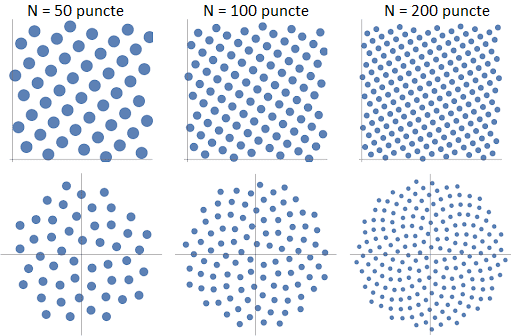
\includegraphics[width=0.92\linewidth]{imagini/fibo.png}
		\caption{Rezultate pentru algoritmul sferei lui Fibonacci \cite{fibo}}
		\label{Fig13}
	\end{figure}
	
	Acest algoritm se bazeaz\u{a} pe o deplasare \^{i}n spiral\u{a} pe suprafa\c{t}a sferei incremental cu unghiul de aur, care este legat de raportul de aur. Dou\u{a} cantit\u{a}\c{t}i, a \c{s}i b, se afl\u{a} \^{i}n raportul de aur dac\u{a}: $\dfrac{a}{b} = \dfrac{a+b}{a} = \varphi$, unde $a>b$, iar acest raport este aproximativ egal cu $\varphi = \dfrac{1+\sqrt{5}}{2}$. Unghiul de aur, $\vartheta$, este definit \^{i}n func\c{t}ie de raportul de aur astfel: $\vartheta = 2\pi(2- \varphi)$. 
	 
	
	\begin{algorithm}
		\caption{Sfera lui Fibonacci}
		\label{fiboLabel}
	\begin{algorithmic}[1]	
		\Procedure{\textit{generare}}{N}
		\State{$\varphi \gets \dfrac{1 + \sqrt{5}}{2}$}
		\State{$\vartheta  \gets 2\pi*(2-\varphi)$}
		\For{$i\gets 0$ to $N$}
		\State{$\theta \gets \sin\left(-1 + \dfrac{2*i}{N + 1}\right)$}
		\State{$\phi \gets \vartheta * i$}
		\State{$dir \gets $ transform\u{a}m (1, $\theta$ \c{s}i $\phi$) \^{i}n coordonate carteziene }
		\State{Scrie dir, direc\c{t}ia pe care se va deplasa viitoarea raz\u{a}}
		\EndFor
		\EndProcedure
	\end{algorithmic}
	\end{algorithm}

	Conform Algoritmului \ref{fiboLabel}, vom distribui razele uniform pe suprafa\c{t}a sferei, urm\^{a}nd ca mai departe s\u{a} gener\u{a}m geometria razelor. 
	
	Bineînțeles, există multiple tehnici de distribuire uniformă a punctelor pe o sferă, precum tehnici de triangulare, metoda respingerii hibercubului (Hypercube Rejection) sau aproximări ale spiralei (Spiral approximations). Tehnica de triangulare presupune crearea unor triunghiuri echilaterale, care să acopere sfera, iar colțul fiecărui triunghi va reprezenta unul dintre punctele distribuite uniform pe sferă. Metoda respingerii hipercubului presupune alegerea unui număr foarte mare de puncte, dar care trebuie să fie mai mare decât numărul dorit și să fie considerate în interiorul unui cub ce conține sfera, după care vom exclude acele puncte care nu se află în sferă. Tehnica aproximării spiralei se referă la alegera unor puncte uniform distribuite care să fie pe o spirală ce se află în jurul sferei. În cazul acestei lucrări se dorește ca distribuirea razelor să se facă uniform cât mai bine și mai rapid. Algoritmul sferei lui Fibonacci permite tocmai acest lucru, întrucât odată cu creșterea numărului de puncte ce se doresc distribuite crește și acuratețea rezultatului. Mai mult de atât, algoritmul are o complexitate bună, liniară, deci codul se va executa rapid.
		
\subsection{Propagarea razelor}

	Dup\u{a} ce am stabilit la pasul anterior punctul de start pentru fiecare raz\u{a}, ne vom preocupa de modul \^{i}n care vor fi generate acestea. Pentru acest lucru este nevoie s\u{a} \c{t}inem cont de c\^{a}teva aspecte precum: legea reflexiei \c{s}i cea a refrac\c{t}iei, care este distan\c{t}a maxim\u{a} pe care o poate acoperi o raz\u{a}, care este num\u{a}rul maxim de reflexii pe care \^{i}l dorim pentru modelul nostru.
	 
	
	Pentru a calcula lungimea unei raze vom folosi distan\c{t}a Euclidian\u{a}:
	\begin{equation}
		d(x,y) = \sqrt{(x-y)^2}
	\end{equation}

	\^{I}n cazul \^{i}n care nu am \c{t}ine cont de lungimea razei am putea ajunge \^{i}n situa\c{t}ia \^{i}n care am crea o raz\u{a} care are mai pu\c{t}ine reflexii dec\^{a}t num\u{a}rul maxim de reflexii, dar care s-ar propaga la infinit pentru c\u{a} nu ar mai \^{i}nt\^{a}lni o suprafa\c{t}\u{a} \^{i}n care s\u{a} se reflecte.
	
	 
	Ca s\u{a} putem crea o raz\u{a} trebuie s\u{a} stabilim de la bun \^{i}nceput \c{s}i care este num\u{a}rul maxim de reflexii pe care dorim s\u{a} \^{i}l permitem. Acest parametru este ales dependent de problema pe care vrem s\u{a} o rezolv\u{a}m, dac\u{a} dorim sa ajungem la o anumit\u{a} performan\c{t}\u{a} sau dorim s\u{a} ob\c{t}inem o solu\c{t}ie c\^{a}t mai apropiat\u{a} de realitate.
	
	 
	Pentru a rezolva problema propag\u{a}rii razelor am folosit urm\u{a}toarea metod\u{a} pus\u{a} la dispozi\c{t}ie de platforma Unity: 
	\begin{itemize}
		\utb 	\textit{public static bool Raycast (Vector3 origin, Vector3 direction, float maxDistance = Mathf.Infinity, int layerMask = DefaultRaycastLayers, QueryTriggerInteraction queryTriggerInteraction = QueryTriggerInteraction.UseGlobal)}, unde \textit{origin} este punctul din care porne\c{s}te raza, \textit{direction} este direc\c{t}ia pe care se deplaseaz\u{a} raza, \textit{maxDistance} este lungimea maxim\u{a} pe care o raz\u{a} o poate avea, \textit{layerMask} este o mască care este utilizată pentru a ignora selectiv collider-urile atunci când este aruncat\u{a} o rază, iar parametrul \textit{queryTriggerInteraction} specific\u{a} dacă această interogare va declanșa o acțiune, pentru a calcula direc\c{t}ia pe care urmeaz\u{a} s\u{a} se deplaseze raza \cite{raycast}.
	\end{itemize}
	 
	Num\u{a}rul maxim de reflexii influen\c{t}eaz\u{a} \^{i}n mod direct at\^{a}t complexitatea, c\^{a}t \c{s}i performan\c{t}a algoritmului. Dac\u{a} vom alege un num\u{a}r foarte mare de reflexii, acesta va duce la cre\c{s}terea timpului de calcul. O raz\u{a} va parcurge o suprafa\c{t}\u{a} mare a camerei atunci c\^{a}nd consider\u{a}m un num\u{a}r mare de reflexii. \^{I}n schimb, dac\u{a} alegem un num\u{a}r prea mic de raze, vom \^{i}nt\^{a}mpina probleme, pentru c\u{a} putem fi pu\c{s}i \^{i}n situa\c{t}ia \^{i}n care nici una dintre raze nu a ajuns pe microfon, ceea ce va avea un impact negativ asupra rezultatului pe care \^{i}l ob\c{t}inem, întrucât nu vom obține rezultate relevante pentru acea încăpere. 
	
	Această tehnică de a trasa razele în încăperi este una foarte potrivită în contextul acestei lucrări tocmai pentru că ne este permisă folosirea razelor pentru a exprima undele sonore. Atunci când discutăm despre frecvențe înalte, undele asocitae au amplitudin mici, ceea ce facilitează folosirea razelor.
	

\subsection{Selec\c{t}ia razelor}

	Unul dintre pa\c{s}ii esen\c{t}iali pentru a ob\c{t}ine performan\c{t}\u{a} este reducerea num\u{a}rului de raze, p\u{a}str\^{a}ndu-le doar pe acelea care ajung pe unul dintre microfoanele plasate \^{i}n \^{i}nc\u{a}pere. Mai mult de at\^{a}t, se pot face \^{i}mbun\u{a}t\u{a}\c{t}iri prin eliminarea duplicatelor. Duplicatele sunt acele raze care dife\u{a} printr-un prag definit, iar p\u{a}strarea acestora cre\c{s}te complexitatea algoritmului, f\u{a}r\u{a} a aduce valoare.
	 
	
	Pentru a selecta doar acele raze care intersecteaz\u{a} microfonul am folost ecua\c{t}ia sferei \cite{intersectie}:
	\begin{equation}
		(x-x_{centru})^2 + (y-y_{centru})^2 + (z-z_{centru})^2 = r^2
	\end{equation}
	\c{s}i a liniei: 
	\begin{equation}
		\begin{cases}
			x = x_1 + x_2 - x_1\\
			y = y_1 + y_2 - y_1\\
			z = z_1 + z_2 - z_1\\
		\end{cases}
	\end{equation}
	 
	
	Substituind $x, y, z$ din ecua\c{t}ia sferei ob\c{t}inem:
	\begin{equation}
		\begin{cases}
			a = (x_2 - x_1)^2 + (y_2 - y_1)^2 + (z_2 - z_1)^2\\
			b = -2[(x_2-x_1)(x_{centru}-x_1) + (y_2 - y_1)(y_{centru} - y_1) + (z_2 - z_1)(z_{centru} - z_1)]\\
			c = (x_{centru}-x_1)^2 + (y_{centru}-y_1)^2 + (z_{centru}-z_1)^2 - r^2\\
		\end{cases}
	\end{equation}
	iar pentru a verifica condi\c{t}ia de intersec\c{t}ie avem urm\u{a}toarele situa\c{t}ii:
	\begin{equation}
		\begin{cases}
			\text{sunt tangente} & b^2-4ac = 0\\
			\text{se intersecteaz\u{a}}& b^2-4ac>0\\
			\text{nu se intersecteaz\u{a}}& b^2-4ac<0\\
		\end{cases}
	\end{equation}
	 
	
	Dou\u{a} raze sunt duplicate dac\u{a} urm\u{a}toarele condi\c{t}ii sunt adev\u{a}rate:
	
	\begin{enumerate}
		\item cele dou\u{a} raze trebuie s\u{a} aib\u{a} acela\c{s}i num\u{a}r de puncte de coliziune;
		
		\item dfieren\c{t}a absolut\u{a} dintre lungimile celor dou\u{a} raze nu trebuie s\u{a} dep\u{a}\c{s}easc\u{a} un prag ales; pragul pe care l-am folosit pentru algoritmul propus a fost $\epsilon = 10^{-2}$;
	\end{enumerate}
	 
	
	\begin{algorithm}
		\caption{Reducerea duplicatelor}
		\label{duplicate}
		\begin{algorithmic}[2]	
			\Procedure{\textit{reducere\_duplicate}}{\textit{raze}}
			\State{$index = 0$}
			\While{$index < no(raze)$}
			\If{$raze_{index}$ \c{s}i $raze_{index+1}$ sunt raze directe} 
			\State{elimin\u{a}m $raze_{index}$ din $raze$}
			\ElsIf{$\mid$distan\c{t}\u{a}($raze_{index}$) - distan\c{t}\u{a}($raze_{index+1}$)$\mid$ $<$ $\epsilon$ \textbf{and} \\ \hspace{2cm} $no(raze_{index}.puncte\_coliziune)= no(raze_{index + 1}.puncte\_coliziune)$}
			\State{elimin\u{a}m $raze_{index}$ din $raze$}
			\State{$index \gets index + 1$}
			\EndIf
			\Else{ $ index \gets index + 1$}
			\EndWhile
			\EndProcedure
		\end{algorithmic}
	\end{algorithm}
	 

	\^{I}n Algoritmul \ref{duplicate} am prezentat modul \^{i}n care a fost realizat\u{a} reducerea de duplicate dup\u{a} ce am considerat doar acele raze care ajung pe microfon. P\^{a}n\u{a} la acest pas am stabilit cum vom distribui razele \^{i}n orice \^{i}nc\u{a}pere, am stabilit care va fi geometria camerei \c{s}i am p\u{a}strat doar acele informa\c{t}ii de interes, adic\u{a} acele raze care ajung pe microfoanele din \^{i}nc\u{a}pere, dar f\u{a}r\u{a} duplicate. 
	
	Lipsa selecției razelor poate crește timpul computațional de la câteva milisecunde, la câteva ore sau chiar zile, în funcție de dimensiunile camerei și numărul de raze distribuit în încăpere. Complexitatea în timp pentru acest pas va fi liniară, întrucât suntem nevoiți să trecem prin toate razele.
	
	Astfel, descrierile urm\u{a}toare prezint\u{a} \^{i}ntr-un mod detaliat modelul fizic \c{s}i matematic pentru algoritmul nostru.

\section{Calcul fizic}

	Am ajuns astfel la etapa de mijloc a modelului, ce propune calcularea c\^{a}torva elemente pentru a putea simula fizica unei \^{i}nc\u{a}peri. La pasul anterior, am realizat geometria unui spa\c{t}iu interior, iar mai departe este nevoie s\u{a} calcul\u{a}m intensit\u{a}\c{t}ile, presiunile, distan\c{t}ele, timpii \c{s}i func\c{t}iile de r\u{a}spuns \^{i}n frecven\c{t}\u{a}, operații pentru care se va păștra complexitatea liniară precum la etapa anterioară. Aceste detalii urmeaz\u{a} s\u{a} fie prezentate mai jos.
	
\subsection{Trecerea \^{i}n domeniul frecven\c{t}elor}
	
	Analiza în domeniul frecvențelor relevă proprietățile semnalului care nu sunt locale în timp, dar răspândite pe un interval, în timp ce analiza timpului este o bază pentru proprietățile locale. Trecerea valorilor din domeniul timpului \^{i}n domeniul frecven\c{t}elor este un pas esen\c{t}ial \^{i}n realizarea algoritmului pentru modelarea acustic\u{a} a spa\c{t}iilor \^{i}nchise, \^{i}ntruc\^{a}t ajut\u{a} la simplificarea calculelor, reduc\^{a}nd astfel timpul computa\c{t}ional pe care \^{i}l necesit\u{a} rularea algoritmului de la câteva minute sau ore la câteva secunde sau milisecunde. Acest procedeu este realizat cu ajutorul Transformatei Rapide Fourier.
	
	Acest pas este unul foarte important pentru ca vine cu câteva avantaje semnificative. Trecerea în domeniul frecvenței permite utilizarea unor componente de analiză spentrală pentru a putea observa semnalul, pentru a extrage caracteristicile acestuia sau pentru a-l clasifica.
	
	În domeniul frecvenței, operația de convoluție este doar o multiplicare, care aduce beneficii enorme, mai ales dacă semnalele au intervale lungi (sau prea multe eșantioane dacă semnalul este digital). Intrarea în domeniul frecvenței este analizarea semnalului dintr-o perspectivă matematică diferită, prin urmare extinde opțiunile de analiză sau procesare a semnalului.
	
\subsection{Calculul intensit\u{a}\c{t}ilor}

	Pentru a calcula intensit\u{a}\c{t}ile pentru fiecare raz\u{a} am folosit Legea P\u{a}tratului Invers \cite{square} care afirm\u{a} ca o m\u{a}rime fizic\u{a} specificat\u{a} este invers propor\c{t}ional\u{a} cu p\u{a}tratul distan\c{t}ei de la sursa acelei m\u{a}rimi fizice. Cauza fundamental\u{a} pentru aceasta poate fi \^{i}n\c{t}eleas\u{a} ca dilu\c{t}ie geometric\u{a} corespunz\u{a}toare radia\c{t}iei punct-surs\u{a} \^{i}n spa\c{t}iul 3D.
	 
	
	Pentru a preveni diluarea energiei în timpul propagării unui semnal, pot fi utilizate anumite metode, cum ar fi un ghid de undă, care acționează ca un canal pentru apă sau modul în care un butoi de pistol restricționează expansiunea gazului fierbinte la o dimensiune pentru a preveni pierderea transferului de energie către un glon\c{t}.
	 
	
	Legea pătratului invers se aplică în general atunci când o anumită forță, energie sau altă cantitate conservată este uniform radiată spre exterior dintr-o sursă punctuală în spațiul 3D. Deoarece suprafața unei sfere este proporțională cu pătratul razei, pe măsură ce radiația emisă se îndepărtează de sursă, aceasta se întinde pe o zonă care crește proporțional cu pătratul distanței de la surs\u{a}. Prin urmare, intensitatea radiației care trece prin orice zonă unitară (direct orientată spre sursa punctuală) este invers proporțională cu pătratul distanței de la sursa punctuală.
	 
	
	Astfel, formula intensit\u{a}\c{t}ii este:
	\begin{equation}
		\frac{I_n}{I_{n+1}} = \frac{d_{n+1}}{d_n}
	\end{equation}
	unde $d_n$ reprezint\u{a} distan\c{t}a de la surs\u{a} p\^{a}n\u{a} la punctul al $n$-lea.
	 
	
	\^{I}n cazul algoritmului ales, atunci c\^{a}nd o raz\u{a} parcurge \^{i}nc\u{a}perea aceasta se love\c{s}te de diferite materiale ce au un factor de absorb\c{t}ie $\alpha$ care variaz\u{a} \^{i}n func\c{t}ie de material. Pentru a putea \c{t}ine cont de fenomenul de absorb\c{t}ie am inclus acest factor \^{i}n formula intensit\u{a}\c{t}ii:
	
	\begin{equation}
		\frac{I_n}{I_{n+1}} = \frac{d_{n+1}}{d_n}(1-\alpha_k)^2
	\end{equation}
	unde $d_n$ are aceea\c{s}i semnifica\c{t}ie ca la pasul anterior, iar $\alpha_k$ reprezint\u{a} coeficientul de absorb\c{t}ie pentru al k-lea material.
	
	În acest mod, în cadrul aplicației vom ține cont de absorbția sunetului în funcție de suprafețele pe care fiecare rază le întâlnește pe traiectul ei, fapt care ne va aduce mai aproape de realitate.

\subsection{Calculul presiunilor}

	Pentru a putea calcula presiunile, ne vom folosi de intensit\u{a}\c{t}ile calculate la pasul anterior, \c{t}in\^{a}nd cont de densitatea aerului \c{s}i de viteza sunetului prin aer. Vom considera c\u{a} densitatea aerului, $\rho_{aer}$, are valoarea $1.2041\dfrac{kg}{m^3}$, iar viteza sunetului prin aer, $c_{aer}$, este $343.21\dfrac{m}{s}$, pentru o temperatur\u{a} constant\u{a} de $20^{\circ}C$.
	 
	
	Prin urmare, formula de transformare a intensit\u{a}\c{t}ii ($I$) \^{i}n presiune ($p$) este:
	\begin{equation}
		p = \sqrt{2 \cdot I\cdot \rho_{aer} \cdot c_{aer}}
	\end{equation}
	 
	
	Nivelul puterii sonore cuantifică energia sonoră total radiată de la un obiect.
	Spre deosebire de presiunea sonoră, intensitatea este independentă de distanța față de sursa de sunet, zona înconjurătoare și alte influențe.
	
	Presiunile, de obicei, au valori pozitive, totuși, există și situații în care acestea pot fi negative. Presiunea este definită ca $\dfrac{F}{A}$, unde $F$ reprezintă forța, iar $A$ reprezintă aria. Dacă o zonă închisă are o presiune mai mare decât aria din jurul ei, gazul/lichidul împinge pentru a ieși, astfel obținem o presiune pozitivă. Atunci când zona închisă are o presiune mai mică decât în jur acea presiune va avea o valoare negativă.

	De exemplu, atunci când suflăm într-un pai se creează o presiune pozitivă în interiorul paiului, pe măsură ce aerul se forțează să iasă din pai. Când tragem dintr-un pai, se creează o presiune negativă în interiorul paiului, și pentru a ușura această presiune, aerul sau băutura se ridică în el.
	
\subsection{Func\c{t}ia de r\u{a}spuns \^{i}n frecven\c{t}\u{a} \c{s}i func\c{t}ia de r\u{a}spuns la impuls}

	Răspunsul la impuls al unui sistem este definit ca semnalul de ieșire care rezultă atunci când un impuls este aplicat la intrarea sistemului. Acesta ne permite să prezicem cum va arăta ieșirea sistemului în domeniul timpului. Dacă putem descompune semnalul de intrare al sistemului într-o sumă de componente, atunci ieșirea este egală cu suma ieșirilor sistemului pentru fiecare dintre aceste componente. Răspunsul la impuls este util deoarece ne permite să calculăm ieșirea sistemelor pentru orice semnal de intrare.

	Pentru fiecare frecven\c{t}\u{a} din interval vom calcula faza \c{s}i magnitudinea:
	\begin{equation}
		\begin{cases}
			t = \dfrac{c_{aer}}{fr}\\
			w = \dfrac{2\pi}{t}\\
			\theta = \arctan{\dfrac{-\sin{w\cdot d}}{\cos{w\cdot d}}}\\
		\end{cases}
	\end{equation}
	unde $fr$ este frecven\c{t}a dat\u{a}, $\theta$ este faza pe care dorim s\u{a} o calcul\u{a}m, iar $d$ este lungimea razei. Ca s\u{a} ob\c{t}inem magnitudinea ne vom folosi de presiunea calculat\u{a} anterior.
	 
	
	\^{I}n urma acestui calcul ob\c{t}inem faza \c{s}i magnitudinea \^{i}n coordonate polare \c{s}i dorim s\u{a} le transform\u{a}m \^{i}n coordonate carteziene. Astfel, vom ob\c{t}ine pentru fiecare frecven\c{t}\u{a} un num\u{a}r complex de magnitudine $m$ \c{s}i faz\u{a} $\theta$. Lista de numere complex\u{a} ob\c{t}inut\u{a} pentru fiecare microfon o vom numi \textit{ecogram\u{a}}.
	 
	
	\^{I}n Figura \ref{Fig15} putem observa care sunt etapele algoritmului. Pentru a putea ajunge la convolu\c{t}ia sunetului trebuie s\u{a} trimitem ca input valori \^{i}n domeniul timpului. Ob\c{t}inerea acestor valori se realizeaz\u{a} prin aplicarea Inversei Transformatei Rapide Fourier peste func\c{t}ia de r\u{a}spuns \^{i}n frecven\c{t}\u{a}.
	 
	
	\begin{figure}[!htb]
		\centering
		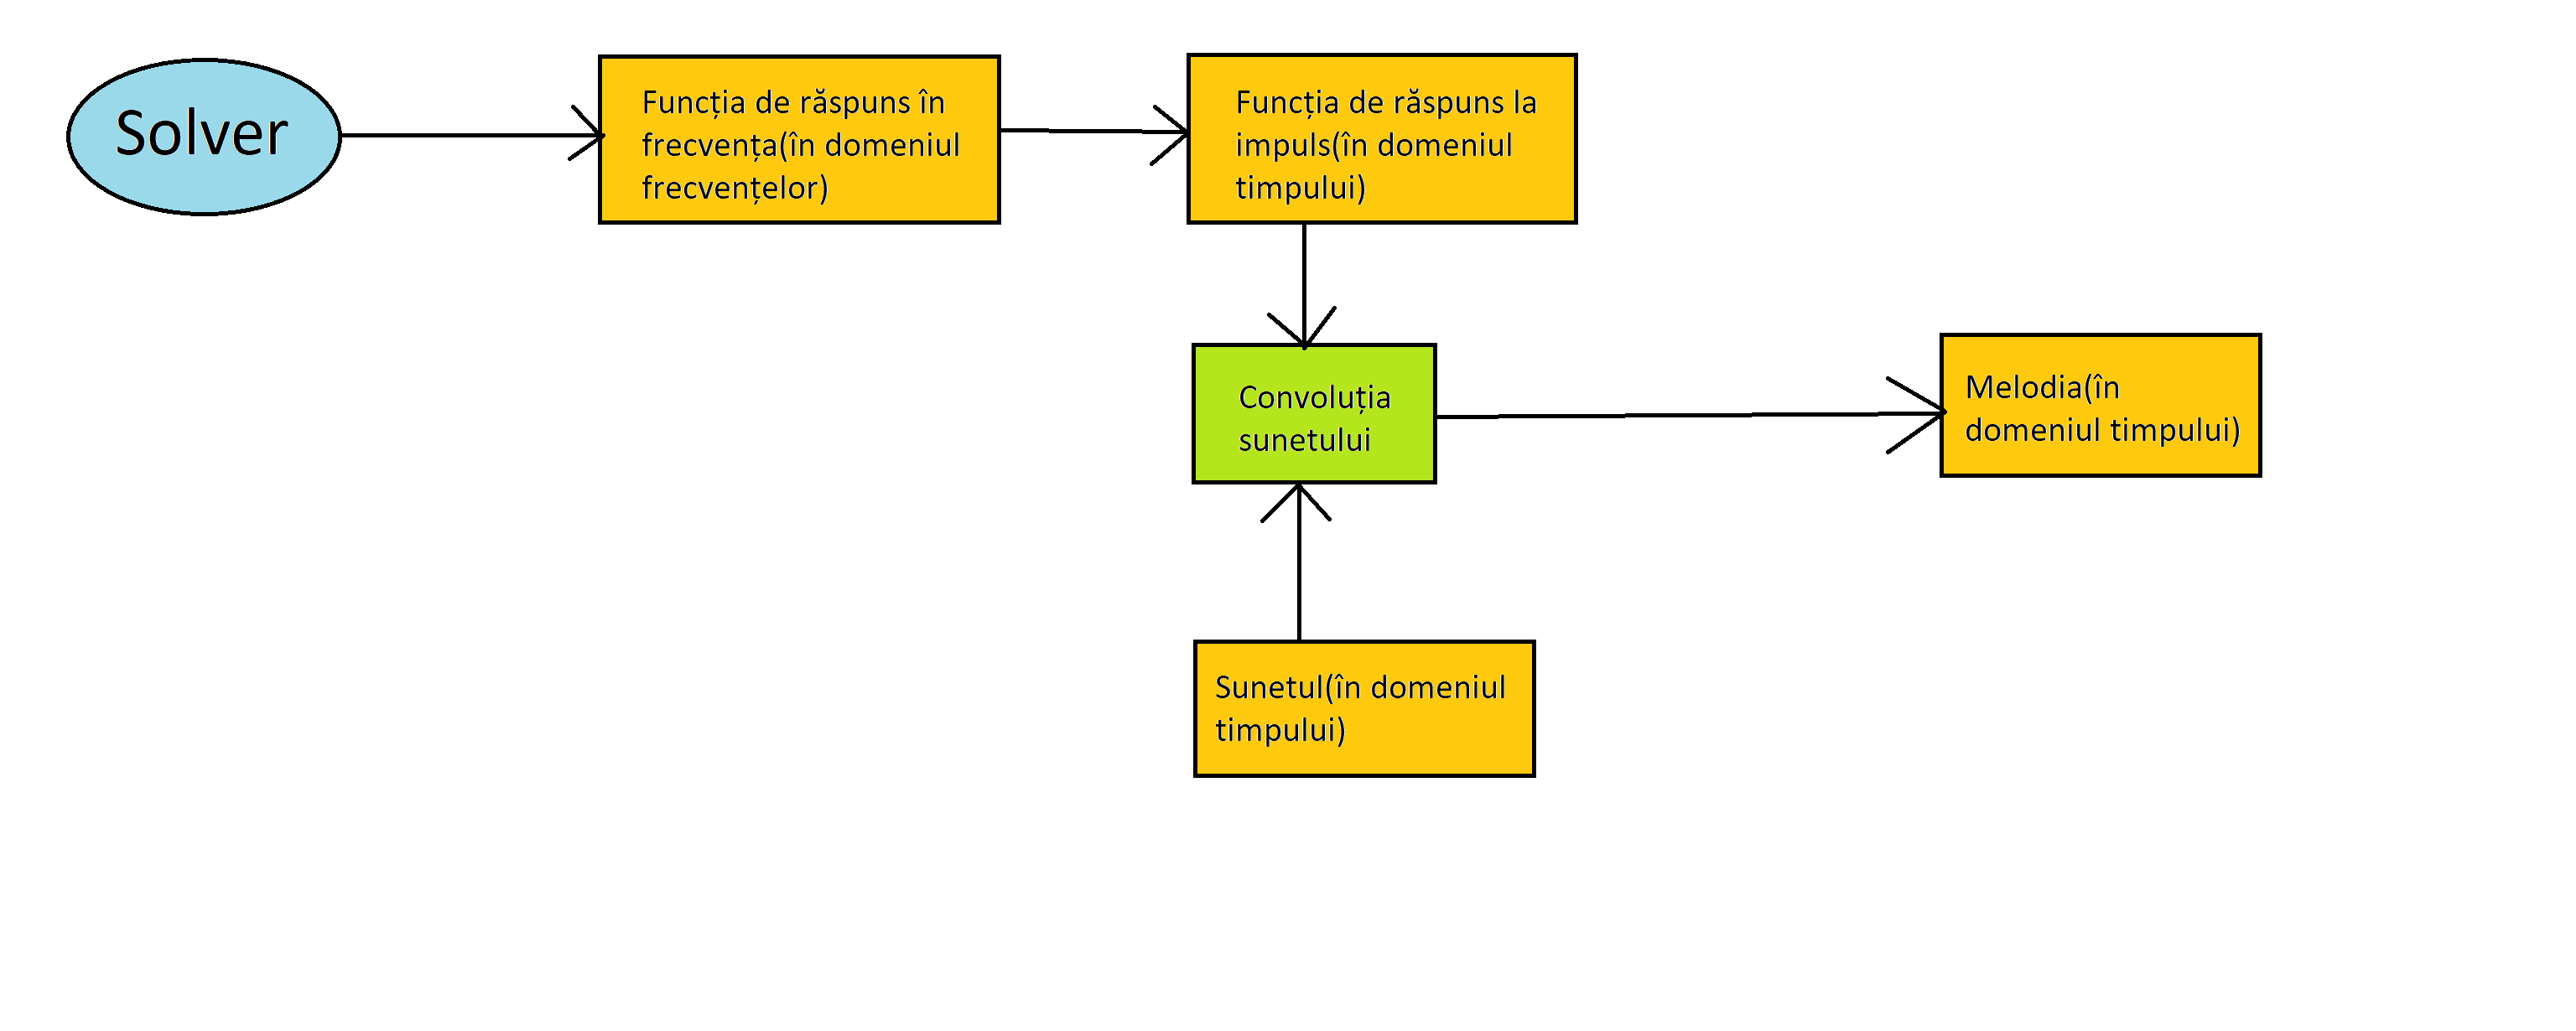
\includegraphics[width=18cm]{imagini/conv.png}
		\caption{Etapele parcurse pentru ob\c{t}inerea sunetului după convoluție}
		\label{Fig15}
	\end{figure}
	
	Func\c{t}ia de r\u{a}spuns la impuls se calculeaz\u{a} pe baza func\c{t}iei de r\u{a}spuns \^{i}n frecven\c{t}\u{a} cu ajutorul Inversei Transformatei Rapide Fourier care va permite trecerea de la domeniul frecven\c{t}elor la domeniul timpului pentru a preg\u{a}ti semnalul de intrare ca mai departe s\u{a} realiz\u{a}m convolu\c{t}ia sunetului.
	Ca s\u{a} putem trece mai departe \c{s}i s\u{a} calcul\u{a}m func\c{t}ia de r\u{a}spuns la impuls trebuie s\u{a} utiliz\u{a}m Algoritmul \ref{frResponse}.
	
	\begin{algorithm}
		\caption{Crearea func\c{t}iei de r\u{a}spuns \^{i}n frecven\c{t}\u{a}}
		\label{frResponse}
		\begin{algorithmic}[3]	
			\Procedure{\textit{r\u{a}spuns\_frecven\c{t}\u{a}}}{\textit{ecograme, microfoane, fr}}
			\State{\textit{r\u{a}spunsFr} $\gets$ dic\c{t}ionar gol}
			\For{$i \gets 0$ to $microfoane$}
			\State{$valori \gets$ list\u{a} numere complexe goal\u{a}}
			\For{$j \gets 0$ to $fr$}
			\State{$sum \gets \sum{ecograme[fr[j]][microfoane[i]]}$}
			\State{$valori.$\textit{adaug\u{a}($sum$)}}
			\EndFor
			\State{\textit{r\u{a}spunsFr[microfoane[i]]}$\gets valori$}
			\EndFor
			\EndProcedure
		\end{algorithmic}
	\end{algorithm}
	 
	
	Acum c\u{a} am ob\c{t}inut r\u{a}spunsul \^{i}n frecven\c{t}\u{a} putem trece la a calcula r\u{a}spunsul la impuls, iar acest lucru se poate face cu ajutorul IFFT, care va permite trecerea de la domeniul frecven\c{t}elor \^{i}napoi la domeniul timpului.
	
	\newpage
\subsection{Calculul distan\c{t}elor}

	Pentru a calcula distan\c{t}ele am folosit formula distan\c{t}ei lui Euler. Am considerat pentru fiecare raz\u{a}, toate punctele de coliziune \c{s}i am calculat lungimile pentru acestea iterativ.
	 
	
	\begin{equation}
		d(p_1, p_2) = \sqrt{(p_{1_x} - p_{2_x})^2 + (p_{1_y} - p_{2_y})^2 + (p_{1_z} - p_{2_z})^2}
	\end{equation}
	 
	
	Prin urmare, lungimea unei raze este calculat\u{a} astfel:
	\begin{equation}
		d_{razei} = \sum_{1}^{N-1}{d(p_i, p_{i+1})}
	\end{equation}
	unde $p_1, p_2, \dots, p_{N}$ sunt punctele de coliziune, iar $N$ reprezint\u{a} num\u{a}rul de puncte de coliziune.

\subsection{Calculul timpilor}

	Calculul timpilor implic\u{a} calculul lungimilor pentru fiecare raz\u{a} \c{s}i viteza sunetului, folosind urm\u{a}toarea formul\u{a}:
	\begin{equation}
		t = \frac{d}{c_{aer}}
	\end{equation}
	unde $t$ este timpul, $d$ reprezint\u{a} distan\c{t}a de la surs\u{a} p\^{a}n\u{a} la ultimul punct de coliziune al razei, iar $c_{aer}$ este viteza sunetului prin aer.

\section{Post-procesarea}

	Funcționalitatea de postprocesare modifică spectrul de frecvență al semnalului audio de intrare. Acest lucru va duce la creșterea anumitor benzi de frecvență, în timp ce altele sunt diminuate sau tăiate. Post-procesarea audio depinde de conținutul audio și presupune aplicarea unor filtre de cele mai multe ori. Post-procesarea audio conține patru mari categorii:
	
	\begin{itemize}
		\utb egalizatoare, care modifică frecvențele
		
		\utb controlul zgomotului, care se ocupă de variația sunetului semnalului audio
		
		\utb sunetul înconjurător, care se ocupă cu crearea unei scene audio realiste și direcționale
		
		\utb efecte audio de sistem, care se ocupă cu îmbunătățirea experienței de utilizare a playerului audio
	\end{itemize}

	Egalizatoarele pot fi utilizate pentru a compensa distorsiunile introduse de sistemul de difuzare a sunetului. Ele pot fi, de asemenea, utilizate pentru a modifica conținutul audio pentru a se potrivi preferințelor ascultătorului.
	
	Nivelul de sunet confortabil pentru conținutul audio depinde, în primul rând de nivelul de zgomotul din jur și, în al doilea rând, de conținutul în sine. În multe aplicații, proiectanții vor găsi necesitatea modificării intensității conținutului audio. Modulul de control al zgomotului măsoară și modifică în consecință intensitatea conținutului audio.

	Astfel, am ajuns \c{s}i la ultima etap\u{a} unde vom aplica opera\c{t}ii de post-procesare pentru a putea asculta sunetul pe microfoanele plasate \^{i}n \^{i}nc\u{a}pere. Astfel, la acest pas vom aplica un algoritm pentru convolu\c{t}ia sunetului ce va fi descris \^{i}n paginile ce urmeaz\u{a}.

\subsection{Convolu\c{t}ia sunetului}

	Convolu\c{t}ia sunetului se face pe baza func\c{t}iei de r\u{a}spuns la impuls. R\u{a}spunsul este alc\u{a}tuit dintr-o list\u{a} de valori reale care sunt transformate \^{i}ntr-un semnal discret. Convolu\c{t}ia presupune un sistem ce prime\c{s}te ca intrare un semanl \c{s}i pe care \^{i}l transform\u{a} pentru a ob\c{t}ine un semnal de ie\c{s}ire. \^{I}n cazul acestui model, semnalul de intrare este func\c{t}ia de r\u{a}spuns la impuls \c{s}i sunetul \^{i}n domeniul timpului, iar ie\c{s}irea este reprezentat\u{a} de valorile reale ale sunetului.
	  
	
	Teoria Fourier spune c\u{a} orice semnal digital poate fi exprimat ca o combina\c{t}ie de sinusoide, din acest motiv prefer\u{a}m s\u{a} realiz\u{a}m calculele \^{i}n domeniul frecven\c{t}elor (este mult mai rapid).
		
	\begin{figure}[!htb]
		\centering
		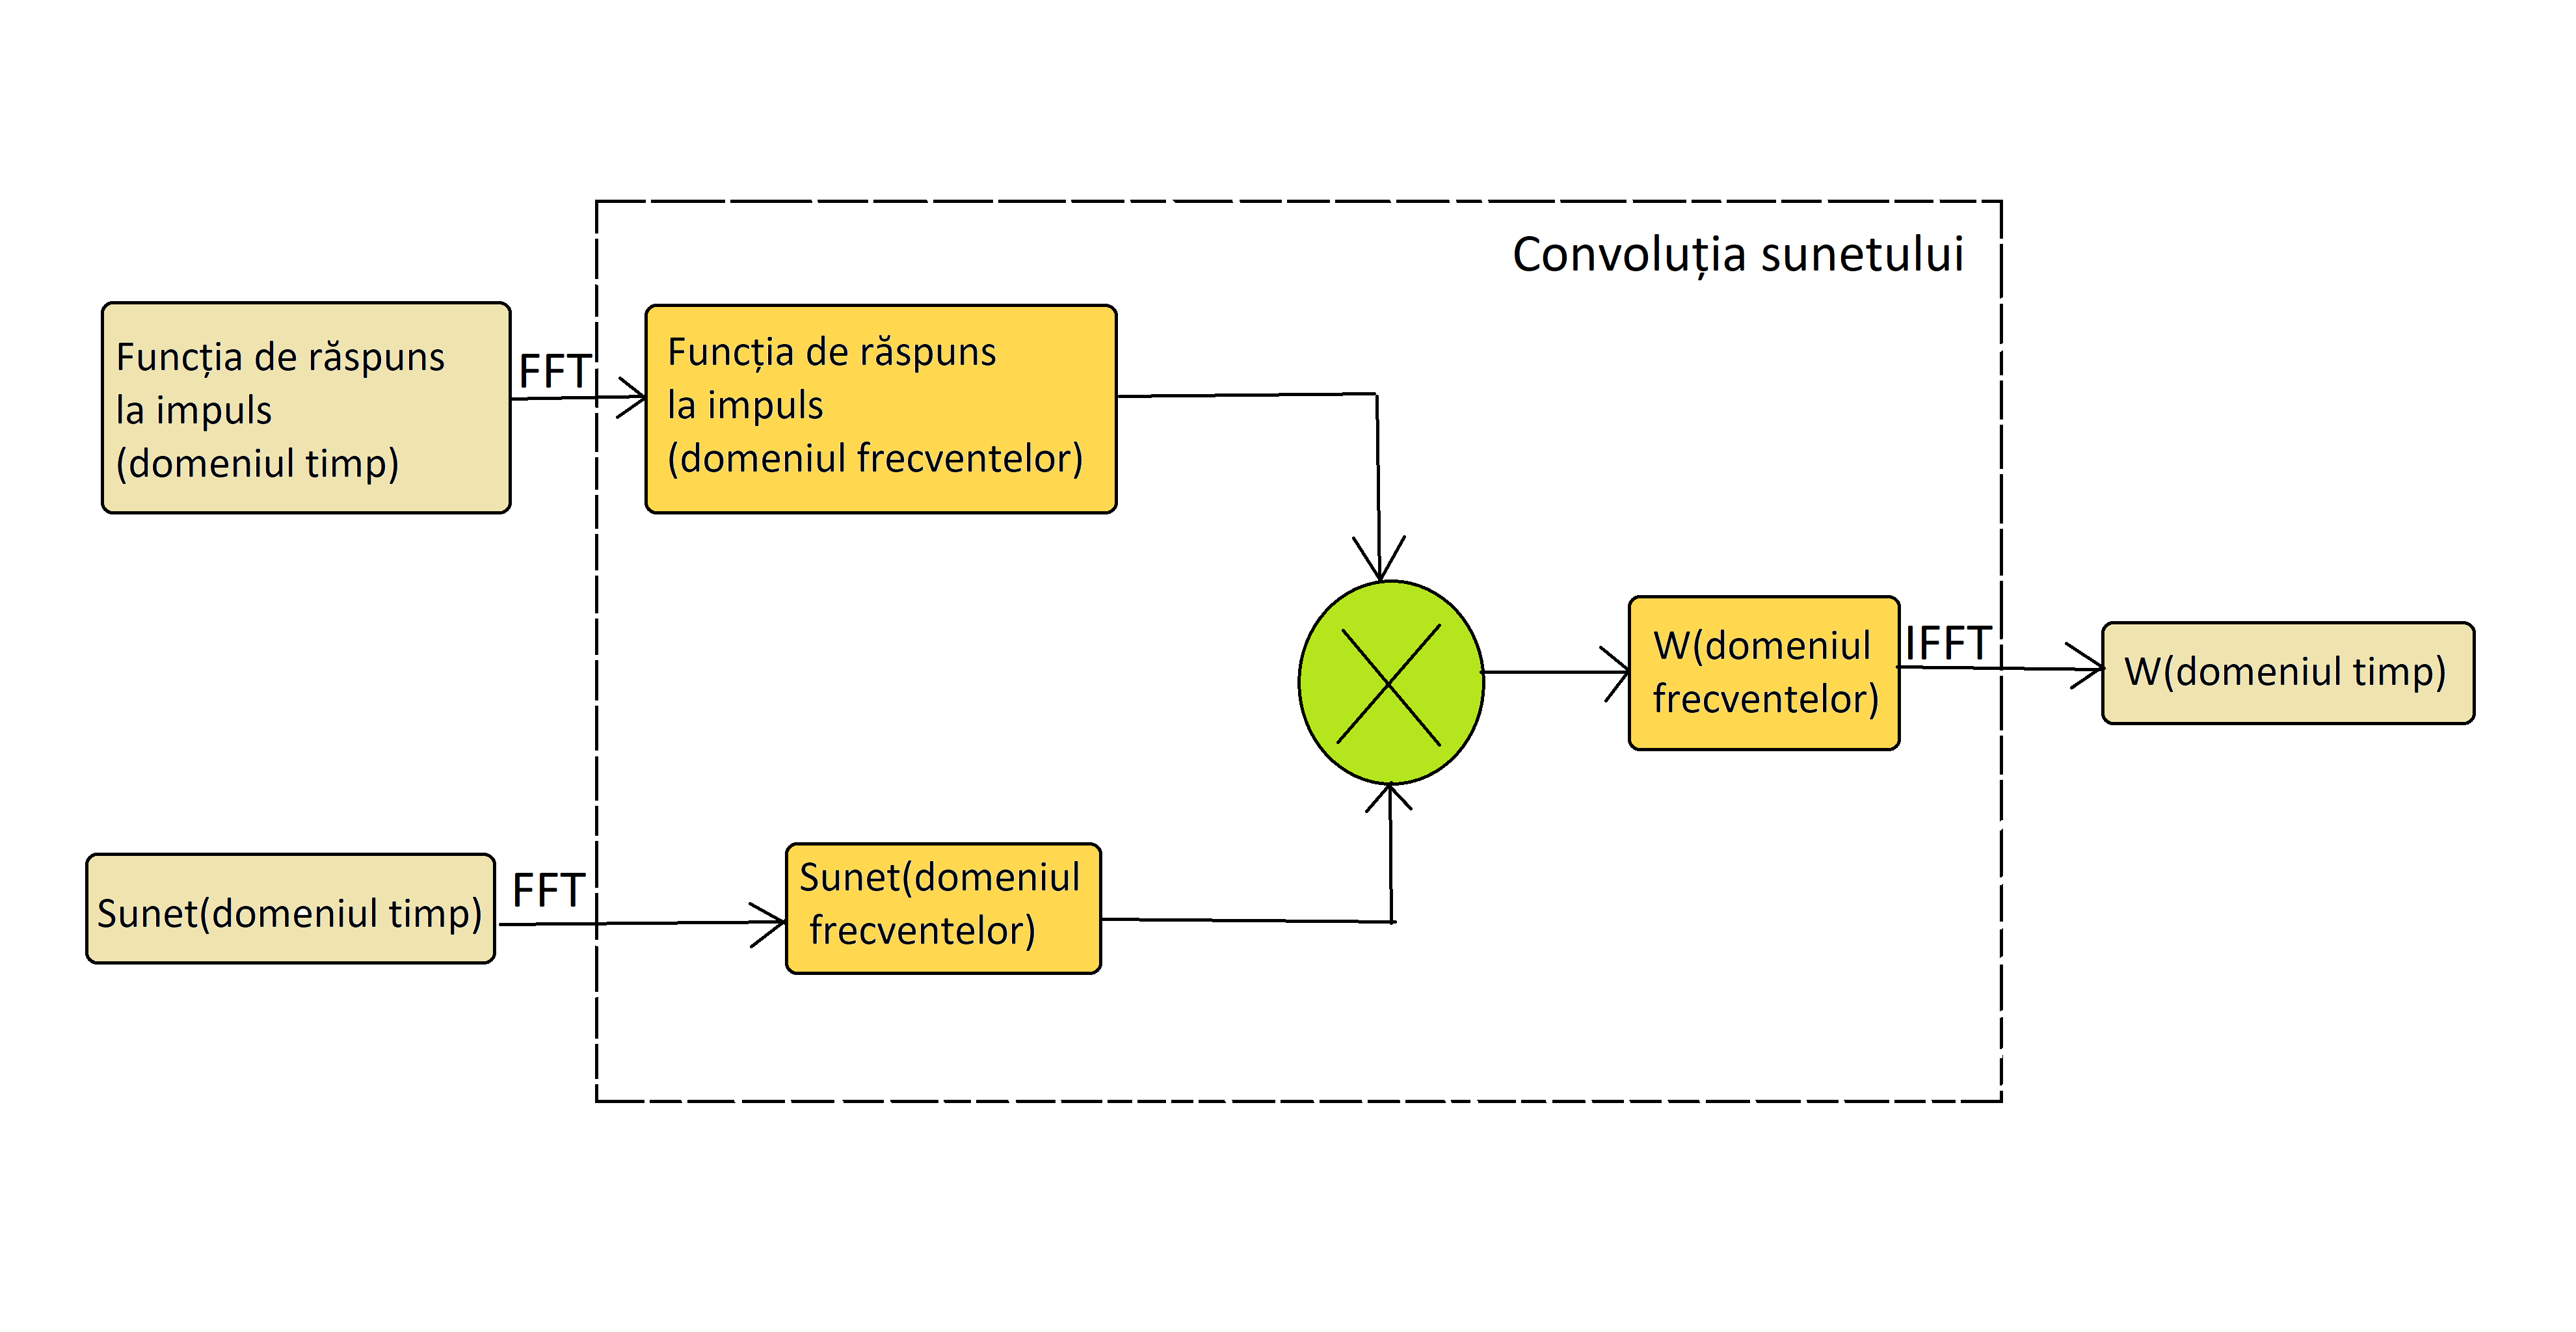
\includegraphics[width=15cm]{imagini/convolutiaSunetului.png}
		\caption{Etapele parcurse pentru convolu\c{t}ia sunetului}
		\label{Fig14}
	\end{figure}

	Precum este descris \c{s}i \^{i}n Figura \ref{Fig14}, convolu\c{t}ia sunetului preia ca intrare func\c{t}ia de r\u{a}spuns la impuls \c{s}i sunetul care a fost difuzat pe sursa audio. Aceste valori sunt \^{i}n domeniul timpului \c{s}i pentru a putea s\u{a} le aplic\u{a}m transform\u{a}rile trebuie s\u{a} trecem \^{i}n domeniul frecven\c{t}elor. Ob\c{t}inem astfel dou\u{a} polinoame ce trebuie \^{i}nmul\c{t}ite. R\u{a}spunsul ob\c{t}inut este \^{i}n domeniul frecven\c{t}elor \c{s}i pentru a calcula ie\c{s}irea trebuie s\u{a} trecem \^{i}napoi \^{i}n domeniul timpului cu ajutor Inversei Transformatei Rapide Fourier. Convolu\c{t}ia sunetului, tranform\u{a}rile din domeniul timpului \^{i}n domeniul frecven\c{t}elor \c{s}i invers au fost realizate cu ajutorul metodelor din NWaves: 
	
	\begin{itemize}
		\utb \textit{DiscreteSignal Operation.Convolve (DiscreteSignal signal, DiscreteSignal kernel);}
		
		\utb \textit{void RealFft.Inverse (float[] re, float[] im, float[] output);}
		
	\end{itemize}

	Semnalul de intrare este sunetul care va fi afectat, în timp ce răspunsul la impuls conține caracteristicile sonore ale spațiului sau obiectului pe care îl vom transmite semnalului de intrare.
	
	Un răspuns la impuls este creat prin redarea unui sunet sau a unui impuls într-un spațiu. Acest impuls poate fi: fie un sunet scurt (un pistol de pornire, un balon care se aprinde etc.), fie un sunet mai susținut ca o sinusoidală (un ton sinusoidal care se ridică prin spectrul de frecvență sonor). Acest impuls produce un instantaneu al ambianței caracteristice a spațiului în conformitate cu acustica unică a spațiului, o ambianță care poate fi capturată.
	
	Microfoanele sunt folosite pentru a înregistra sunetul rezultat. Având în vedere impulsul inițial, putem vedea cum acustica spațiului/obiectului afectează timbrul sunetului rezultat.
	
	În mod ideal, impulsul inițial ar fi editat din înregistrare, lăsând doar răspunsul acustic al spațiului. Acest lucru ar lăsa un semnal pur al spațiului, mai degrabă decât să includă un alt sunet cu spațiul.
	
	În esență, convoluția este procesul de multiplicare a spectrelor de frecvență ale celor două surse audio - semnalul de intrare și răspunsul la impuls. Procedând astfel, frecvențele care sunt partajate între cele două surse vor fi accentuate, în timp ce frecvențele care nu sunt partajate vor fi atenuate. Acesta este motivul pentru care semnalul de intrare capătă calitățile sonore ale răspunsului la impuls, deoarece frecvențele caracteristice din răspunsul la impuls comun în semnalul de intrare sunt amplificate.

	Procedura este semnificativ mai eficientă din punct de vedere al timpului de calcul decât celelalte două etape, deoarece folosind Transformata Fourier Rapidă (FFT) ajungem la $n\log_2n$ operații necesare pentru a realiza convoluția sunetului.